\section{Precision of Indoor Location}\label{sec:estimoteprecision}
Another core part of our system is indoor location. 
For the ``point-to-select'' part of our system to work as intended, we need high indoor precision. 
In \Cref{sec:indoor-positioning} we mentioned that Estimote claims the accuracy to be less than \num{5} meters.
In this section we test if that is actually the case, or even if we can achieve better results than that. 
We test this by comparing the position we get from the application to the actual position we have in the room. 
We test in with the following four settings:
\begin{enumerate}
    \item Room 1: $5 \times 5$ meter room with no walls
    \item Room 2: $8 \times 8$ meter room with no walls
    \item Room 3: Outside in a $17.9 \times 17.9$ meter square with no walls
    \item Room 4: $4.9 \times 9.95$ meter room
\end{enumerate}

We test in different settings to measure if, and how much, 
the size of the room matters in terms of accuracy. 
We decided to test outside in an area where there were none or few WiFi signals,
as WiFi shares the same same radio frequency as BLE (\SI{2.4}{\GHz}). 
We have performed tests both with and without movement. 

\subsection{Room 1}
Room 1 and Room 2 have been setup in an auditorium. 
We used tables to simulate walls, 
and we placed the beacons on chairs on top of the tables. 
The setup can be seen in \Cref{fig:audtest} and illustrated in \Cref{fig:audtestsetup}. 
\todo[author=Thalley]{Insert number of 2.4 GHz access points}

\begin{figure}[!htb]
    \centering
    \includegraphics[width=\textwidth]{drawings/audtest}
    \caption{The setup for Room 1 and Room 2. Room 1 is marked as the inner (blue) square and is $5 \times 5$ meters. Room 2 is marked as the outer (red) square and is $8 \times 8$ meters. The Estimote beacons are placed on the chairs.}
    \label{fig:audtest}
\end{figure}

\begin{figure}[!htb]
    \centering
    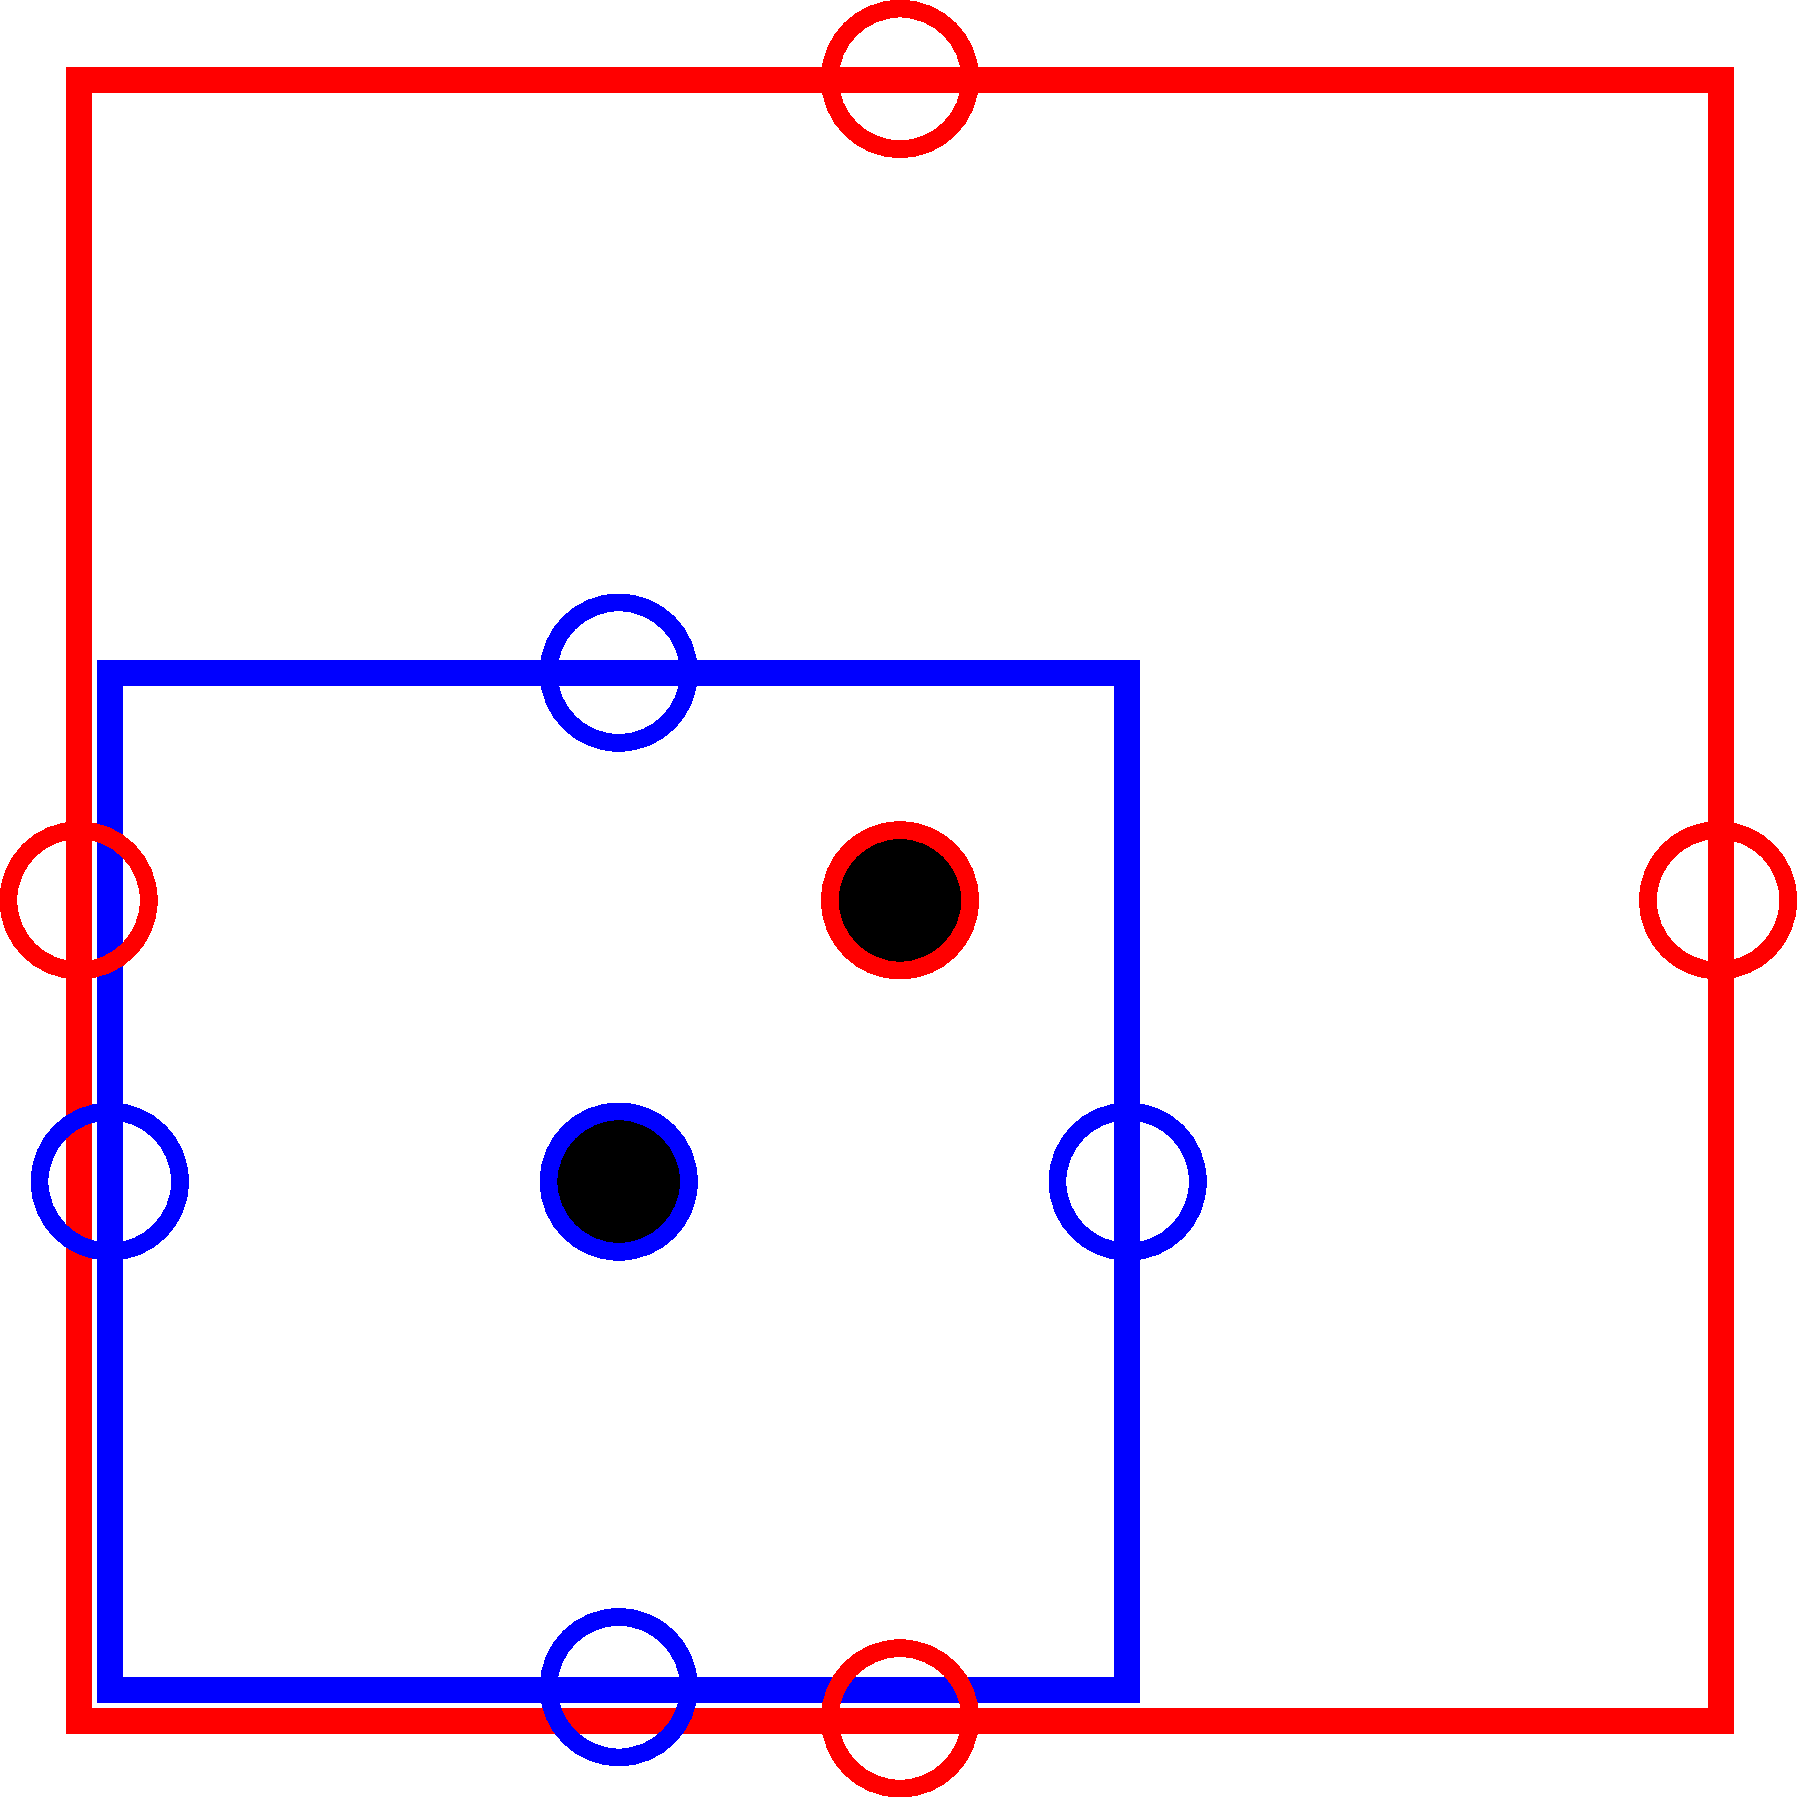
\includegraphics[width=0.6\textwidth]{drawings/audtestsetup}
    \caption{The setup for Room 1 and Room 2 (illustration of \Cref{fig:audtest}). Room 1 is marked as the inner (blue) square and is $5 \times 5$ meters. Room 2 is marked as the outer (red) square and is $8 \times 8$ meters. The rings shows the position of the beacons. The filled circles shows where the the phone is placed to obtain the position (only for the non-moving tests).}
    \label{fig:audtestsetup}
\end{figure}

\FloatBarrier
\subsection{Room 2}

\subsection{Room 3}

\subsection{Room 4}

\subsection{Conclusion}


We setup a [SIZE OF ROOM] room, with [NUMBER OF BEACONS]. 
The room is illustrated by \Cref{fig:precisiontest}. 
In \Cref{fig:precisiontest} you can also see small spots. 
These spots is the known locations where we are going to perform the precision tests. 
We randomly walk between these spots [NUMBER OF TIMES] and find the mean error rate.
\begin{figure}[!htb]
    \centering
    \todo[author=Thalley]{Insert figure}
    \caption{Illustration of room used for indoor location precision test}
    \label{fig:precisiontest}
\end{figure}

The mean error rate that we found is [RESULT]. 

\subsection{Precision of Indoor Location Conclusion}
From the results, we can conclude that... \todo[author=Thalley]{Write conclusion of precision test based on results}

